\documentclass[conference]{IEEEtran}
\IEEEoverridecommandlockouts
% The preceding line is only needed to identify funding in the first footnote. If that is unneeded, please comment it out.
%Template version as of 6/27/2024

\usepackage{cite}
\usepackage{amsmath,amssymb,amsfonts}
\usepackage{algorithmic}
\usepackage{graphicx}
\usepackage{textcomp}
\usepackage{xcolor}
\usepackage{multirow}
\usepackage{booktabs}
\usepackage{array}
\def\BibTeX{{\rm B\kern-.05em{\sc i\kern-.025em b}\kern-.08em
    T\kern-.1667em\lower.7ex\hbox{E}\kern-.125emX}}
\begin{document}

\title{Lightweight Four-State Driver Monitoring from Facial Geometry and Eye-Mouth Crops with INT8 Post-Training Quantization}

\author{\IEEEauthorblockN{Vivek Parashar}
\IEEEauthorblockA{\textit{Dept. of Computer Science and Engineering (SCOPE)} \\
\textit{VIT Bhopal University}\\
Kothri Kalan, Madhya Pradesh, India \\
vivekparashar@vitbhopal.ac.in}
\and
\IEEEauthorblockN{Aayushi Vinod}
\IEEEauthorblockA{\textit{Dept. of Computer Science and Engineering (SCOPE)} \\
\textit{VIT Bhopal University}\\
Kothri Kalan, Madhya Pradesh, India \\
aayushi.vinod2507@gmail.com}
\and
\IEEEauthorblockN{Payoshi Gupta}
\IEEEauthorblockA{\textit{Dept. of Computer Science and Engineering (SCOPE)} \\
VIT Bhopal University\\
Kothri Kalan, Madhya Pradesh, India \\
guptapayoshi2016@gmail.com}
\and
\IEEEauthorblockN{Anshika Singh}
\IEEEauthorblockA{\textit{Dept. of Computer Science and Engineering (SCOPE)} \\
VIT Bhopal University\\
Kothri Kalan, Madhya Pradesh, India \\
anshikasinghh504@gmail.com}
\and
\IEEEauthorblockN{Tanisha}
\IEEEauthorblockA{\textit{Dept. of Computer Science and Engineering (SCOPE)} \\
VIT Bhopal University\\
Kothri Kalan, Madhya Pradesh, India \\
lambatanisha021@gmail.com}
\and
\IEEEauthorblockN{Amit Yadav}
\IEEEauthorblockA{\textit{Dept. of Computer Science and Engineering (SCOPE)} \\
VIT Bhopal University\\
Kothri Kalan, Madhya Pradesh, India \\
amityadav022117@gmail.com}
}

\maketitle

\begin{abstract}
Camera-based driver monitoring should recognize different kinds of inattention, not only drowsiness, and must run on low-cost CPUs. We study a four-state formulation (Focused, Drowsy, Yawning and Looking Away) built on MediaPipe Face Mesh, where each frame is described by nine geometric features and by 64$\times$64 crops of the eyes and mouth. Using a subject-disjoint protocol that combines the MRL Eye, YawDD datasets and our own webcam recordings and YouTube videos, we compare a rule-based baseline, a geometry-only network, a crop-only CNN, a fusion network, a MobileNetV3 variant and a focal-loss variant. A small crop CNN with about 138k parameters performs the best (macro-F1 0.637, accuracy 91.2\%), narrowly ahead of a 3.7k-parameter geometry network (0.633); fusion (0.595), MobileNetV3 (0.561) and focal-loss-based CNN (0.576) do not help. Focused and Yawning classes are recognized well, whereas Drowsy is the weakest class (best F1 0.41) and is most likely confused with Looking Away. Label quality matters: 84\% of the test frames from yawning clips show a closed mouth and a CNN trained and evaluated without relabeling them reaches only 0.449 macro-F1 on its own, noisier label set. Manual refinement of 620 Drowsy and Looking Away labels from our own recordings gave a macro-F1 of 0.431 under the same setting, i.e., no measurable gain. Post-training INT8 quantization shrinks CNN model size by 2.9$\times$ (0.57 to 0.20 MB) with unchanged macro-F1 (0.637 to 0.638), but gives no speed-up on an x86 laptop CPU, where Face Mesh dominates the end-to-end time (about 88--95 FPS); it degrades MobileNetV3 (macro-F1 0.561 to 0.480). Under synthetic low light, macro-F1 of the FP32 CNN falls from 0.633 (L1) to 0.466 (L3), although at L3 a face is still found in  only 5\% of the frames.
\end{abstract}

\begin{IEEEkeywords}
driver monitoring, drowsiness detection, facial landmarks, MediaPipe, label noise, post-training quantization, edge computing.
\end{IEEEkeywords}

\section{Introduction}

The lack of attention of the driver is one of the leading causes of road accidents and a camera facing the driver is one of the few sensors that can observe them without any contact. Driver drowsiness is the most studied case \cite{fonseca2025,fu2024,fu2024app}, but a useful monitor also has to notice yawning, a sign of fatigue and a driver who looks away from the road, for example, at a phone; distracted driving is a research area in its own right, with dedicated datasets and reviews \cite{wang2023,dontoh2025}. Deploying such a monitor in a vehicle imposes a second requirement: inference has to run in real time on a low-power CPU without a GPU.
Three practical problems stand in the way. First, no public dataset covers all the states of interest. MRL Eye \cite{mrl, fusek2018} offers infrared eye crops with open/closed labels, YawDD \cite{yawdd} offers in-car videos of yawning and normal driving and neither contains looking away behavior. Moreover, YawDD labels whole videos as yawning although most of their frames show normal driving or talking, which introduces label noise \cite{mujtaba2025}. Second, frames from the same person are nearly identical, so a random frame-level split leaks identity into the test set and inflates accuracy; this kind of leakage is a recognized cause of over-optimistic results in machine learning studies \cite{kapoor2023}. Third, deep models are often evaluated in FP32 on a workstation, which says little about their cost on an embedded CPU, although recent work already targets resource-constrained deployment of drowsiness detectors \cite{alajlan2023}.
This paper studies these problems with a deliberately small system. Our contributions are:
\begin{enumerate}
    \item A four-state formulation and a subject-disjoint data protocol which combines MRL Eye, YawDD dataset and our own webcam recordings and YouTube videos with automatic labeling and a leakage test.
    \item A feature pipeline based on MediaPipe Face Mesh that generates nine geometric features and two image crops and a rule-based baseline whose thresholds are calibrated on a validation split.
    \item A comparison of geometry-only, crop-only and fused networks, a MobileNetV3 encoder and a focal-loss variant of CNN model on the same split and seed, evaluated with macro-F1 and per-class F1 and the selection of a small crop CNN as the deployment model.
    \item Evidence on label quality: most frames in yawning clips show a closed mouth and a CNN trained and evaluated on the unrefined labels reaches only 0.449 macro-F1 on that noisier label set (not directly comparable with the refined-label scores).
    \item A quantization-friendly architecture, a post-training INT8 procedure and a benchmark protocol (latency, throughput, CPU, memory, size, accuracy under normal and low light).
    \item A real-time demonstration application, available as a desktop (OpenCV) and a local browser (Flask) version that share one temporal decision layer based on consecutive-frame and PERCLOS-style rules.
\end{enumerate}
We also report negative findings, because with few own subjects they matter as much as the headline numbers: fusion, a larger MobileNetV3 encoder and focal loss all fail to improve on the simple crop CNN and Drowsy remains hard to detect by any model.



\vspace{0.2cm}
\section{Related Work}

\subsection{Cues for Drowsiness and Inattention}\label{sec:cues}
PERCLOS, the proportion of time the eyes are closed over a window, is a long-established measure of alertness \cite{perclos}. A common frame-level proxy for eye closure is the Eye Aspect Ratio (EAR), calculated from facial landmarks \cite{soukupova2016}. Yawning is commonly detected using the Mouth Aspect Ratio (MAR) and gaze or attention away from the road is identified using head pose. Recent surveys \cite{albadawi2022,fonseca2025,fu2024,fu2024app} group approaches into behavioral (camera), physiological and vehicle-based methods and describe the trade-off between simple, interpretable features and learned models. The survey of Fu et al.\ \cite{fu2024} also names model compression as a remedy for the limits of embedded hardware, which motivates the quantization study in this paper.
\newline Landmark-based systems remain popular because they are cheap. Webcam systems based on EAR and facial landmarks reach high accuracy in good light but degrade at night \cite{rao2024}, low-cost systems with dynamic thresholds have been built for under US\$50 \cite{khan2026} and infrared systems combine landmark-based eye-closure detection with head-pose recognition to detect both drowsiness and inattention \cite{kim2023}. Far-infrared cameras have also been used to detect yawning, head drooping and head pose together \cite{knapik2024}. Most work treats drowsiness as a single binary decision; joint classification of several driver states from face data has been explored more recently \cite{akhmedov2025} and our four-state formulation follows the same idea with a lightweight landmark-based pipeline. For distraction, reviews report that vision-only models reach high accuracy but generalize poorly to real driving conditions \cite{dontoh2025} and that most studies were run in simulators or laboratories rather than in vehicles \cite{john2024}.

\subsection{Datasets}
NTHU-DDD \cite{weng2016} is a widely used benchmark of simulated driving with drowsy and non-drowsy labels. YawDD \cite{yawdd} contains videos of drivers who are talking, yawning or driving normally, recorded with mirror-mounted and a dash-mounted camera. MRL Eye \cite{mrl,fusek2018} contains about 85,000 infrared eye images from 37 subjects with eye-state, glasses, reflection and lighting annotations. Newer resources include 100-Driver, a large dataset for distracted-driver classification \cite{wang2023} and YawDD+, which re-annotates YawDD at frame level and shows that video-level labels add noise to yawning detection \cite{mujtaba2025}. Our work uses MRL Eye and YawDD and adds own recordings and YouTube videos to cover the looking-away and drowsy states.

\subsection{Landmarks, Efficient Networks, Imbalance and Quantization}
MediaPipe \cite{lugaresi2019} provides real-time Face Mesh landmarks \cite{kartynnik2019} that run on a CPU. For image models, MobileNetV3 \cite{howard2019} is a standard efficient backbone and newer members of the family such as MobileNetV4 target a wide range of mobile hardware \cite{qin2024}, but the hard-swish activations and squeeze-and-excitation blocks of MobileNetV3 are difficult to quantize in eager mode. Class imbalance is commonly handled by class weighting or by the focal loss \cite{lin2017}, which down-weights easy examples. Ghosh et al.\cite{ghosh2024} survey these and other remedies for deep networks. Integer-arithmetic-only inference \cite{jacob2018} and the practical recipes in \cite{krishnamoorthi2018} make post-training static quantization a low-effort way to reduce latency and model size and Rokh et al.~\cite{rokh2023} survey post-training and quantization-aware methods for image classification. However, the benefit of INT8 is not guaranteed: measured speed-ups depend on the integer kernels and instructions of the target hardware \cite{shin2026} and layers differ in how sensitive they are to quantization, which mixed-precision methods exploit \cite{ramp2026}. We follow the standard recipe and choose a plain Conv BatchNorm ReLU encoder so that module fusion is applied cleanly. Finally, clip-level labels such as ours can contain wrong labels and learning from noisy labels is an active research area \cite{song2023}; Sections~\ref{sec:refine} and~\ref{sec:manualeffect} examine this effect directly.



\vspace{0.2cm}
\section{Datasets and Protocol}

\begin{table}[t]
\caption{Data Sources}
\label{tab:data_sources}
\centering
\small
\renewcommand{\arraystretch}{1.3}
\begin{tabular}{|p{1.4cm}|p{3.0cm}|p{1.0cm}|p{1.5cm}|}
\hline
Source & Content & Subjects & Used for \\
\hline
MRL Eye &
Infrared eye crops, open/closed &
37 &
Eye-encoder pre-training \\
\hline
YawDD (Mirror) &
In-car videos: normal, talking, yawning &
90 &
Yawning, Focused \\
\hline
Own webcam &
30 sec clips of all four states, 640$\times$480, 30 fps &
10 &
All four classes \\
\hline
YouTube Videos &
30 sec to 2 min clips of Drowsy and Looking Away classes &
8 &
Drowsy and Looking Away\\
\hline
\end{tabular}
\end{table}

\subsection{Data Sources}\label{sec:sources}
Table~\ref{tab:data_sources} lists the four sources. MRL Eye provides eye-state labels only; it is used to initialize the eye encoder. YawDD (Mirror set) provides Yawning and Focused frames. Our own custom recordings are the only source of all the four classes; Drowsy and Looking Away frames come from them and from the YouTube clips.

\subsection{Own Recordings}\label{sec:own}
Each participant recorded 30-second clips of one behavior at a time: Focused (looking at the screen, normal blinking), Drowsy (slow blinks, eyes closed for three to four seconds and head drooping), Yawning (mouth wide open for two to four seconds) and Looking Away (head turned or looking down at a phone or to the side). Seven subjects were recorded in normal room lighting and three in a dark room lit only by a study lamp, and where applicable with and without glasses. The participants gave their informed consent. The person, class, lighting and glasses status are encoded in the video file name, so that labels are generated automatically. The first and last second of every clip are discarded because they contain transitions.

\subsection{Frame Extraction and Labels}\label{sec:labels}
We keep every second frame of each clip (frame step~2) to avoid thousands of near-duplicate images. YawDD clips are labeled from their file names: yawning clips as Yawning, normal and talking clips as Focused. Own-clip frames and YouTube video frames inherit the class of the clip. Only a few seconds of a yawning clip contain an open mouth, so after feature extraction we relabel every Yawning frame as Focused where mouth aspect ratio is below a cutoff of 0.35. Section~\ref{sec:refine} quantifies the effect of this refinement. Frames in which Face Mesh finds no face are excluded from training and testing and flagged in the feature file.

\subsection{Manual Refinement of Drowsy and Looking Away Labels}\label{sec:manualref}
In addition to the automatic refinement of Yawning labels to the Focused class, we conducted a manual label-refinement experiment on our own webcam recordings of Drowsy and Looking Away classes of each person. In the original labeling procedure, all extracted frames inherited the class that was assigned to the corresponding video in the file name. This assumption can introduce incorrect labels when the driver's behavior changes within a clip. For example, frames in a Drowsy clip may show the driver with eyes open, while the frame in the Looking Away clip may show the driver facing forward.
\newline To address this mislabeling, we manually reviewed frames originally labeled as Drowsy or Looking Away in the own-recording dataset. Each reviewed frame was assigned a corrected label based on its visible behavior, using the four existing classes: Focused, Drowsy, Yawning and Looking Away. The review resulted in 620 label changes: 458 Drowsy-to-Focused, 86 Drowsy-to-Looking Away, 24 Looking Away-to-Drowsy and 52 Looking Away-to-Focused. The original image paths, subject identifiers and train-validation-test assignments were kept the same. The 7,569 frames labeled Drowsy or Looking Away in our own webcam recordings (3,783 and 3,786 frames) were reviewed by a single person, and the 620 changes affect 8.2\% of them; YouTube frames were not re-labeled.
\newline The refined annotations were saved separately from the original labels. We then regenerated the geometric features and eye-mouth crops and trained a separate Crop CNN using the refined feature file. The original dataset and model checkpoints were preserved for comparison.

\subsection{Subject-Disjoint Split}\label{sec:split}
Because consecutive frames of one person are nearly identical, splitting by frame would place the same face in training and test sets. We therefore assign whole subjects to the training, validation and test splits (70/15/15), separately for each source, with a fixed random seed (42). The labeling script asserts that no subject appears in two splits and a unit test repeats the check. Table~\ref{tab:subject_distribution} gives the number of subjects per split and Table~\ref{tab:manual_refinement} the resulting frame counts. For MRL Eye the split is used only for eye-encoder pre-training.

\begin{table}[t]
\caption{Distribution of Subjects Across Dataset Splits}
\label{tab:subject_distribution}
\centering
\begin{tabular}{|l|r|r|r|r|}
\hline
\textbf{Dataset} & \textbf{Train} & \textbf{Validation} &
\textbf{Test} & \textbf{Total} \\
\hline
MRL Eye & 25 & 6 & 6 & 37 \\
Own Recordings & 6 & 2 & 2 & 10 \\
YawDD & 62 & 14 & 14 & 90 \\
YouTube & 6 & 1 & 1 & 8 \\
\hline
\textbf{Total} & \textbf{99} & \textbf{23} &
\textbf{23} & \textbf{145} \\
\hline
\end{tabular}
\end{table}

Two properties of this split shape every result below. The data are highly imbalanced: Focused frames make 61.5\% of the labeled frames in Table~\ref{tab:manual_refinement} (79,592 of 129,377; before face filtering and MAR relabeling) and 87.2\% of the evaluated test frames (19,075 of 21,874; after face filtering and MAR relabeling), so a classifier that always answers Focused scores highly on accuracy. Drowsy and Looking Away come only from own recordings and YouTube clips (5,731 and 6,844 frames in total), from 10 own subjects and 8 YouTube subjects. In the test split, Looking Away comes from the 2 own test subjects only and the single YouTube test subject contributes only Drowsy; in the validation split the single YouTube subject contributes only Looking Away and the own recordings contain no Focused frames. The Drowsy and Looking Away results, therefore, rest on very few people.



\begin{table*}[!t]
\centering
\caption{Labeled frames per class by source and split, before and after manual refinement (before face filtering and before MAR relabeling of Yawning frames, so the Yawning columns are unaffected by the refinement).}
\label{tab:manual_refinement}
\renewcommand{\arraystretch}{1.2}
\setlength{\tabcolsep}{4pt}
\resizebox{\textwidth}{!}{%
\begin{tabular}{|c|c||r|r|r|r|r||r|r|r|r|r|}
\hline
\multirow{2}{*}{\textbf{Split}} &
\multirow{2}{*}{\textbf{Source}} &
\multicolumn{5}{c||}{\textbf{Before Manual Refinement}} &
\multicolumn{5}{c|}{\textbf{After Manual Refinement}} \\
\cline{3-12}
& &
\textbf{Focused} &
\textbf{Drowsy} &
\textbf{Yawning} &
\textbf{Looking Away} &
\textbf{Total} &
\textbf{Focused} &
\textbf{Drowsy} &
\textbf{Yawning} &
\textbf{Looking Away} &
\textbf{Total} \\
\hline
\multirow{4}{*}{\textbf{Train}}
& Own
& 1,052 & 2,207 & 2,198 & 2,211 & 7,668
& 1,377 & 1,901 & 2,198 & 2,192 & 7,668 \\

& YawDD
& 52,904 & 0 & 22,616 & 0 & 75,520
& 52,904 & 0 & 22,616 & 0 & 75,520 \\

& YouTube
& 0 & 1,542 & 0 & 1,500 & 3,042
& 0 & 1,542 & 0 & 1,500 & 3,042 \\

& \textbf{All}
& \textbf{53,956} & \textbf{3,749} & \textbf{24,814} & \textbf{3,711} & \textbf{86,230}
& \textbf{54,281} & \textbf{3,443} & \textbf{24,814} & \textbf{3,692} & \textbf{86,230} \\

\hline

\multirow{4}{*}{\textbf{Val}}
& Own
& 0 & 840 & 737 & 839 & 2,416
& 15 & 752 & 737 & 912 & 2,416 \\

& YawDD
& 12,218 & 0 & 4,891 & 0 & 17,109
& 12,218 & 0 & 4,891 & 0 & 17,109 \\

& YouTube
& 0 & 0 & 0 & 1,558 & 1,558
& 0 & 0 & 0 & 1,558 & 1,558 \\

& \textbf{All}
& \textbf{12,218} & \textbf{840} & \textbf{5,628} & \textbf{2,397} & \textbf{21,083}
& \textbf{12,233} & \textbf{752} & \textbf{5,628} & \textbf{2,470} & \textbf{21,083} \\

\hline

\multirow{4}{*}{\textbf{Test}}
& Own
& 317 & 736 & 634 & 736 & 2,423
& 487 & 610 & 634 & 692 & 2,423 \\

& YawDD
& 13,101 & 0 & 6,134 & 0 & 19,235
& 13,101 & 0 & 6,134 & 0 & 19,235 \\

& YouTube
& 0 & 406 & 0 & 0 & 406
& 0 & 406 & 0 & 0 & 406 \\

& \textbf{All}
& \textbf{13,418} & \textbf{1,142} & \textbf{6,768} & \textbf{736} & \textbf{22,064}
& \textbf{13,588} & \textbf{1,016} & \textbf{6,768} & \textbf{692} & \textbf{22,064} \\

\hline

\multicolumn{2}{|c|}{\textbf{Total}}
& \textbf{79,592} & \textbf{5,731} & \textbf{37,210} & \textbf{6,844} & \textbf{129,377}
& \textbf{80,102} & \textbf{5,211} & \textbf{37,210} & \textbf{6,854} & \textbf{129,377} \\

\hline
\end{tabular}%
}
\end{table*}


\subsection{Synthetic Low-Light Test Sets}\label{sec:lowlight}
To test robustness we darken the test split with three fixed levels. For a pixel intensity $x\in[0,1]$,
\begin{equation}
x' = \operatorname{clip}\!\bigl(b\,x^{\gamma} + \varepsilon,\,0,\,1\bigr),\qquad \varepsilon\sim\mathcal{N}\!\bigl(0,(\sigma/255)^2\bigr),
\label{eq:lowlight}
\end{equation}
with $(b,\gamma,\sigma)=(0.60,1.5,3)$ for L1, $(0.35,2.0,8)$ for L2 and $(0.15,2.5,15)$ for L3. The levels are generated once with a fixed seed so that all models are compared on identical images. Synthetic darkening does not reproduce real sensor noise, so three of our ten own subjects were recorded in a dark room lit only by a study lamp and the other seven in normal room lighting; the own recordings therefore contain real low-light frames. A separate evaluation on real low-light recordings is left to future work. Low light is a known weakness of landmark-based systems \cite{rao2024}, which is why infrared and far-infrared cameras are used in some designs \cite{kim2023, knapik2024}; we only evaluate an RGB webcam.



\vspace{0.2cm}
\section{Method}

\begin{figure*}[t]
    \centering
    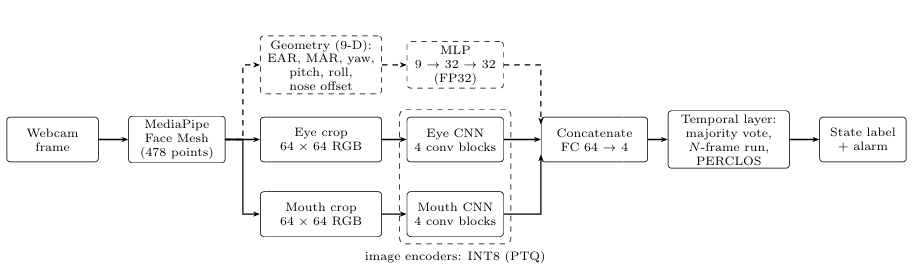
\includegraphics[width=\textwidth]{pipeline.png}
    \caption{Pipeline of the monitor. A single Face Mesh pass feeds two image branches and, in the geometry-only and fusion variants of the ablation, a geometry branch (dashed). The selected deployment model uses only the solid path; its image encoders are quantized to INT8.}
    \label{fig:pipeline}
\end{figure*}

\subsection{Facial Features}\label{sec:feat}
Fig.~\ref{fig:pipeline} gives an overview of the system: one Face Mesh pass per frame feeds the feature and crop branches, a classifier head predicts one of four states and a temporal layer turns the per-frame predictions into a stable state and an alarm. Face Mesh returns 478 landmarks per frame. The eye aspect ratio of one eye is 
\begin{equation}
\mathrm{EAR} = \frac{\|p_2 - p_6\| + \|p_3 - p_5\|}
{2\|p_1 - p_4\|}
\label{eq:ear}
\end{equation}
where $p_1, \ldots, p_6$ are six landmarks around the eye, with $p_1$ and $p_4$ at the corners; it approaches zero as the eye closes. We store the left and right values and their mean. The mouth aspect ratio averages three vertical inner-lip distances $h_i$ and divides by the mouth width $w$:
\begin{equation}
\mathrm{MAR} = \frac{1}{3w} \sum_{i=1}^{3} h_i
\label{eq:mar}
\end{equation}
which rises as the mouth opens. Head pose is estimated with a perspective-n-point solver (OpenCV~\cite{opencv}) from six landmarks (nose tip, chin, outer eye corners, mouth corners) and a generic 3-D face model, with the focal length set to the image width and no lens distortion. The rotation is converted to yaw, pitch and roll in degrees. Finally, the nose offset from the center of the landmark bounding box, normalized by its size, provides two further values. The feature vector therefore has nine entries:
$(\mathrm{EAR}_L, \mathrm{EAR}_R, \overline{\mathrm{EAR}}, \mathrm{MAR}, \mathrm{yaw}, \mathrm{pitch}, \mathrm{roll}, \Delta_x, \Delta_y)$.
The same extract function is used for dataset building and by the live application, so that preprocessing cannot differ between training and deployment.

\subsection{Eye and Mouth Crops}\label{sec:crops}
From the same landmarks we crop a square region around both eyes and another around the mouth, each enlarged by a factor of 1.6 and resized to $64 \times 64$ RGB.

\subsection{Rule-Based Baseline}\label{sec:rule}
The baseline is a decision list with four thresholds:
\begin{equation}
\hat{y} =
\begin{cases}
\text{Looking Away} & | \text{yaw} | > \tau_y \lor |\text{pitch}| > \tau_p, \\
\text{Yawning} & \text{else if } \mathrm{MAR} > \tau_m, \\
\text{Drowsy} & \text{else if } \overline{\mathrm{EAR}} < \tau_e, \\
\text{Focused} & \text{otherwise}.
\end{cases}
\label{eq:driver_state}
\end{equation}
The thresholds are found by exhaustive grid search that maximizes macro-F1 on the validation split only 
(EAR: $0.12$--$0.30$, MAR: $0.20$--$0.80$,
yaw: $15^\circ$--$45^\circ$,
pitch: $10^\circ$--$35^\circ$),
and are then frozen and applied once to the test and low-light sets. The selected thresholds are $\tau_e=0.26$, $\tau_m=0.35$, $\tau_y=45^\circ$ and $\tau_p=35^\circ$. The yaw and pitch values lie at the upper edge of their search ranges, so the grid may be too narrow for them, and $\tau_m$ equals the 0.35 cutoff used to relabel Yawning frames (Section~\ref{sec:labels}).

\subsection{Networks}\label{sec:networks}
All learned models share the same building blocks. The image encoder is a four-block CNN: each block is a $3 \times 3$ convolution with stride 2, BatchNorm and ReLU, with 16, 32, 64 and 64 channels, followed by global average pooling and a 64-unit fully connected layer. Separate encoders process the eye and mouth crops. The geometry branch is a two-layer perceptron $(9 \rightarrow 32 \rightarrow 32)$.
The classifier head maps the concatenated representation to 64 units (ReLU, dropout 0.2) and then to four logits. Crop normalization and feature standardization, using the training-set mean and standard deviation, are part of the model, so that a stored checkpoint is self-contained. We train the following variants (Table~\ref{tab:test_results}):
\textit{Geometry} (the perceptron and head only),
\textit{Crop CNN} (two encoders and head),
\textit{Fusion} (all branches) and
\textit{MobileNetV3}, in which each encoder is replaced by
the MobileNetV3-Small \cite{howard2019} feature extractor with
global average pooling and a 64-unit projection
(ImageNet-pretrained).
A further variant, \textit{CNN + focal}, uses the Crop CNN
with a different loss (Section~\ref{sec:train}).

\subsection{Training}\label{sec:train}
The default objective is a class-weighted cross-entropy with weights
$w_c = N/(C\,n_c)$ where $N$ is the number of training frames, $C$ = 4 and $n_c$ the count of class $c$, class weighting and focal loss are the two remedies for imbalance that we compare \cite{lin2017,ghosh2024}. For the focal-loss variant we use
\begin{equation}
\mathcal{L}_{\text{focal}} = -w_y (1-p_y)^\gamma \log p_y,
\quad \gamma = 2
\label{eq:focal_loss}
\end{equation}
where $p_y$ is the predicted probability of the true class $y$ and $w_y$ is the same class weight \cite{lin2017}. We do not use class-balanced resampling: all runs use standard shuffling. Optimization uses Adam \cite{kingma2015} (learning rate $10^{-3}$, weight decay $10^{-4}$), a cosine learning-rate schedule \cite{loshchilov2017}, batch size 128 and 25 epochs, in PyTorch \cite{paszke2019}. The checkpoint with the best validation macro-F1 is kept. To prepare for dim lighting, half of the crops in every batch are randomly darkened with Eq.~(\ref{eq:lowlight}) (with $\gamma \sim U(1, 2.2),\ b \sim U(0.3, 1)$ and noise standard deviation $\sim U(0, 0.06))$; the geometric features are not modified.
The eye encoders of the Crop CNN and Fusion models are initialized from a network trained for three epochs to classify MRL eye images as open or closed; because these images are single infrared eyes, the initialization is only a weak prior for our RGB two-eye crops. All results use one seed (42).

\subsection{Temporal Decision Layer}\label{sec:temporal}
A single frame cannot separate a blink from falling asleep, so the application smooths the per-frame predictions. The displayed state is the majority vote over the last nine frames. A drowsiness alarm is raised when $N$ = 45 consecutive frames (about 1.5 s at 30 fps) are predicted Drowsy, or when a PERCLOS-style measure, the share of Drowsy predictions in a 30\,s window, exceeds 0.20 after at least 10 s of data. The run counter is reset after 15 non-drowsy frames and the alarm is cleared only when PERCLOS falls below 80\% of its trigger value, which avoids flickering. If no face is found for 15 consecutive frames, the state becomes Looking Away. The frame-count rules are defined in frames, so their delay in seconds depends on the processing frame rate (1.5 s corresponds to 45 frames only at 30 fps).

\subsection{Quantization and Benchmark Protocol}\label{sec:quantprotocol}
We apply post-training static quantization \cite{jacob2018,krishnamoorthi2018,rokh2023} to the two image encoders of the selected Crop CNN. In eager mode, Conv-BN-ReLU triplets are fused, observers are inserted, and the encoders are calibrated with 400 training samples (half of them darkened) before conversion to INT8; the small classifier head remains in FP32. We use the fbgemm backend on x86 and qnnpack on ARM. For the MobileNetV3 encoder we use FX graph mode, because hard-swish and squeeze-and-excitation blocks are difficult to quantize in eager mode.
Each configuration is benchmarked in a fresh process with batch size one, one CPU thread, 50 warm-up and 500 timed iterations, reporting mean and 95th-percentile latency. CPU utilization and resident memory are sampled with psutil, model size is the checkpoint size on disk, and accuracy is measured on the test split and on L1--L3. We report model-only latency (crops in, logits out) separately from end-to-end latency (frame in, state out), because Face Mesh is not quantized and dominates the latter.



\vspace{0.2cm}
\section{Experimental Results}

\begin{table}[t]
\caption{Test results (21,874 frames, single run, seed 42). Parameters are trainable weights, excluding BatchNorm statistics. Bold marks the best value in each column among the first five rows.}
\label{tab:test_results}
\centering
\scriptsize
\renewcommand{\arraystretch}{1.2}
\setlength{\tabcolsep}{3pt}
\begin{tabular}{|p{2cm}|c|c|c|c|c|c|c|}
\hline
\multirow{2}{*}{\textbf{Model}} &
\multirow{2}{*}{\textbf{Params}} &
\multirow{2}{*}{\textbf{Acc.}} &
\multirow{2}{*}{\textbf{Macro-F1}} &
\multicolumn{4}{c|}{\textbf{F1 per class}} \\
\cline{5-8}
& & & &
\textbf{Foc.} &
\textbf{Drow.} &
\textbf{Yawn.} &
\textbf{Away.} \\
\hline
Geometry & 3.7K & 0.849 & 0.633 & 0.930 & \textbf{0.406} & \textbf{0.948} & 0.248 \\
\hline
Crop CNN (sel.) & 138K & \textbf{0.912} & \textbf{0.637} & \textbf{0.966} & 0.182 & 0.863 & \textbf{0.537} \\
\hline
Fusion & 142K & 0.893 & 0.595 & 0.964 & 0.084 & 0.946 & 0.386 \\
\hline
MobileNetV3 & 1.94M & 0.889 & 0.561 & 0.956 & 0.042 & 0.908 & 0.338 \\
\hline
CNN + focal & 138K & 0.891 & 0.576 & 0.954 & 0.076 & 0.823 & 0.451 \\
\hline
Rule-based & -- & 0.685 & 0.535 & 0.802 & 0.301 & 0.913 & 0.124 \\
\hline
CNN, no relabel$^{*}$ & 138K & 0.608 & 0.449 & 0.715 & 0.088 & 0.472 & 0.524 \\
\hline
CNN, manual ref.$^\dagger$ & 138K & 0.604 & 0.431 & 0.724 & 0.122 & 0.452 & 0.427 \\
\hline
\end{tabular}

\vspace{3pt}
\parbox{\columnwidth}{\scriptsize
$^{*}$Evaluated against the unrefined labels (13,403 / 1,028 / 6,743 / 700 frames), so not comparable with other models (Section~\ref{sec:refine}).\\
$^\dagger$Trained and evaluated on the manually refined labels with MAR relabeling disabled; its reference is the no-relabel row (Section~\ref{sec:manualeffect}).
}
\end{table}

\begin{figure*}[t]
    \centering
    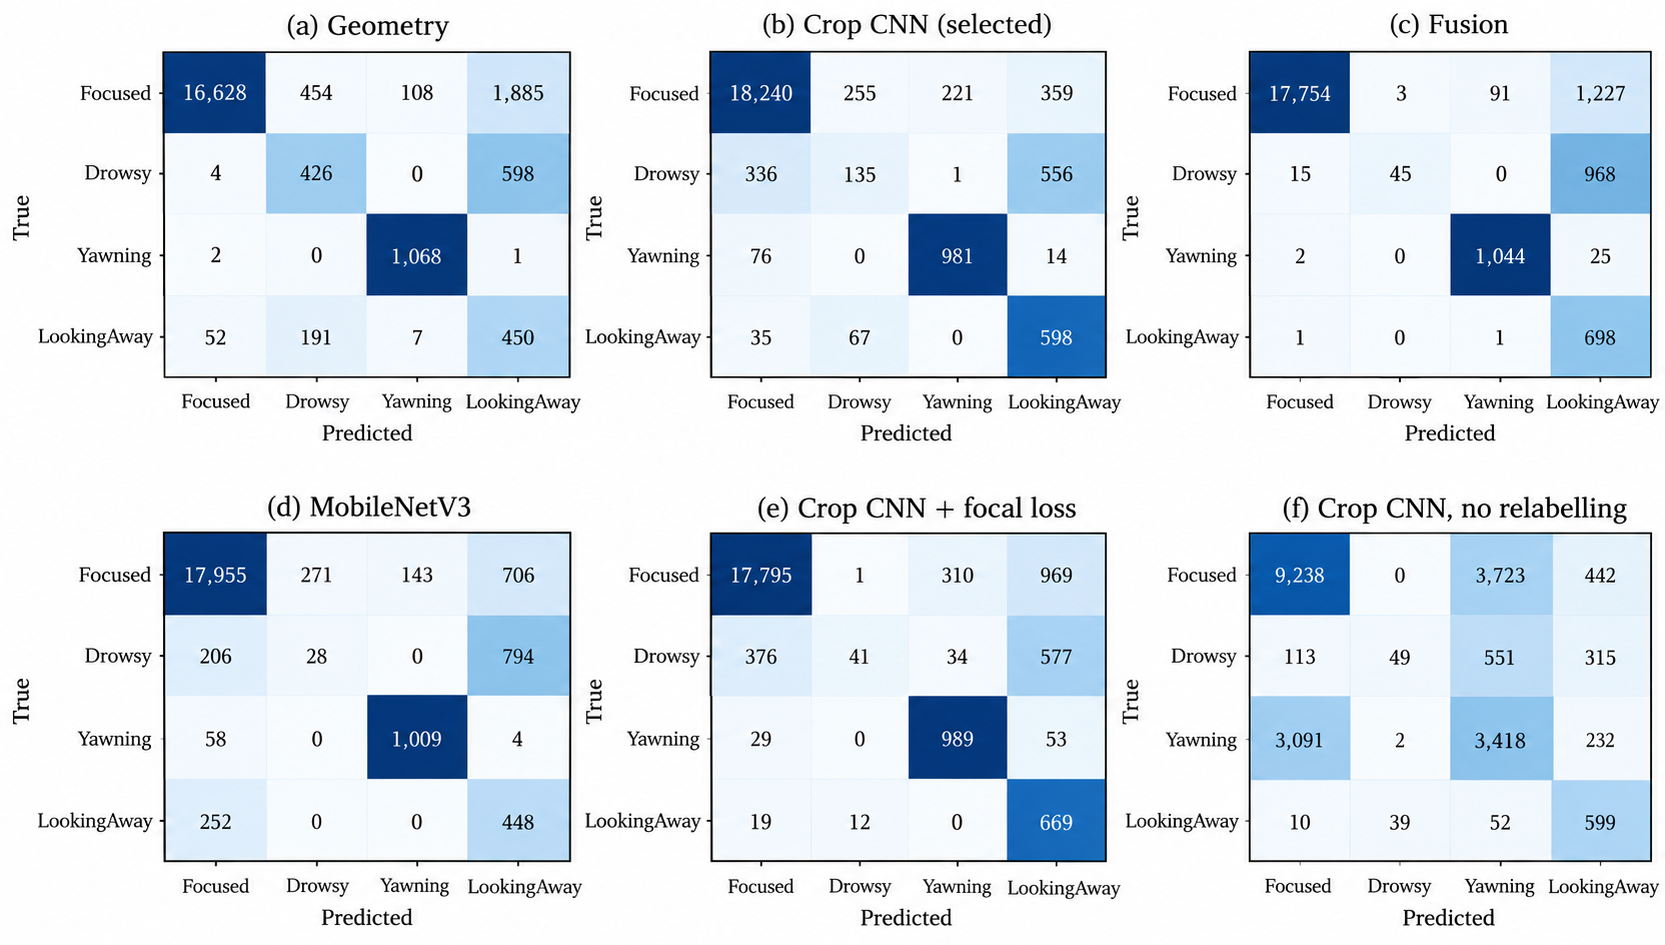
\includegraphics[width=\textwidth]{confusion_matrices.png}
    \caption{Confusion matrices on the test split (counts; shading shows the row-normalized share). Panels (a)--(e) use the refined labels. Panel (f) is the Crop CNN trained and tested without relabeling closed-mouth frames in yawning clips, so its Yawning and Focused rows contain different frames.}
    \label{fig:confusion_matrices}
\end{figure*}

\subsection{Setup and Metrics}\label{sec:setup}
All numbers are computed on the held-out test split (21,874 frames; 190 of the 22,064 test frames had no detected face and were excluded), with hyper-parameters, thresholds and checkpoints chosen on the validation split. Because 87.2\% of test frames are Focused, accuracy is a weak indicator. We treat macro-F1 and per-class F1 as the main metrics and report accuracy for completeness. Following the advice to state exactly which macro-F1 is meant \cite{opitz2024}, we compute it as the unweighted mean of the four per-class F1 scores. Software versions follow the repository requirements (PyTorch 2.4.1, MediaPipe 0.10.14, OpenCV 4.10); hardware is 12th Gen Intel Core i5-1235U CPU, 8 GB RAM, Microsoft Windows 11 64-bit OS.

\begin{table*}[!t]
\centering
\caption{FP32 versus INT8 benchmark (batch size 1, one thread).
Latency, p95, FPS, CPU and RSS are measured for the model alone
on CPU; for the Crop CNN these are medians of three runs and for
MobileNetV3 a single run. Macro-F1 is on the clean test split and on L3.}
\label{tab:fp32_int8_benchmark}
\footnotesize
\setlength{\tabcolsep}{5pt}
\renewcommand{\arraystretch}{1.15}
\begin{tabular}{|l|c|c|c|c|c|c|c|c|c|}
\hline
\textbf{Model} &
\textbf{Precision} &
\textbf{Size (MB)} &
\textbf{Latency (ms)} &
\textbf{p95 (ms)} &
\textbf{FPS} &
\textbf{CPU (\%)} &
\textbf{RSS (MB)} &
\textbf{Macro-F1} &
\textbf{Macro-F1 L3} \\
\hline
Crop CNN & FP32 & 0.572 & 1.33 & 2.41 & 752 & 95.8 & 194 & 0.637 & 0.466 \\
\hline
Crop CNN & INT8 (eager) & 0.195 & 2.10 & 4.00 & 476 & 94.4 & 130 & 0.638 & 0.464 \\
\hline
MobileNetV3 & FP32 & 7.99 & 5.00 & 5.91 & 200 & 99.4 & 226 & 0.561 & 0.625 \\
\hline
MobileNetV3 & INT8 (FX) & 2.54 & 9.14 & 19.49 & 109 & 97.9 & 181 & 0.480 & 0.061 \\
\hline
\end{tabular}
\end{table*}

\subsection{Comparison of Models}\label{sec:compare}
Table~\ref{tab:test_results} and Figs.~\ref{fig:confusion_matrices} and~\ref{fig:test_f1_comparison} compare the models. The Crop CNN has the best accuracy (0.912, above the 0.872 majority-class rate), the best macro-F1 (0.637) and the best Focused (0.966) and Looking Away (0.537) F1. The 3.7k-parameter geometry network is effectively tied on macro-F1 (0.633) and is the best at Drowsy (F1 0.406, recall 41\%) and, together with fusion, at Yawning (0.948). However, its accuracy (0.849) is below the majority-class rate, because it labels 1,885 Focused frames (9.9\%) as Looking Away.
Adding the geometry features to the crops did not help. The fusion network reaches 0.595 macro-F1, 0.042 below the Crop CNN. Its losses are in Drowsy (F1 0.084) and Looking Away (0.386): it predicts Looking Away for 968 of the 1,028 Drowsy frames (94\%), and for 1,227 Focused frames, so its Looking Away recall is 99.7\% but its precision only 24\%. A MobileNetV3-Small encoder, with roughly an order of magnitude more parameters, is worse than the small CNN (0.561), and sends 794 Drowsy frames (77\%) to Looking Away. Replacing the weighted cross-entropy by focal loss (\(\gamma = 2\), same class weights) lowers macro-F1 from 0.637 to 0.576: Looking Away recall rises to 96\% but its precision falls to 29\%, Drowsy and Yawning both worsen. The differences between the geometry network and the Crop CNN (0.004) are far smaller than the variation we would expect between seeds and subjects; the gaps to fusion, MobileNetV3 and the focal-loss variant (0.04--0.08) are larger, but each result comes from a single run. The rule-based baseline (0.535) has the second-best Drowsy F1 (0.301), ahead of every image model, which supports an eye-closure cue for Drowsy; its Yawning score is circular, because its MAR threshold (0.35) equals the relabeling cutoff, and that of the geometry network is partly so (Section~\ref{sec:refine}).
\newline
\textbf{Drowsy is mostly mistaken for Looking Away.} Every neural model sends more than half of the Drowsy frames to Looking Away: 54\% for the Crop CNN (556 of 1,028), 58\% for the geometry network, 56\% for the focal-loss variant, 77\% for MobileNetV3 and 94\% for fusion (Fig.~\ref{fig:confusion_matrices}). The selected Crop CNN recognizes only 13\% of Drowsy frames (recall), although its Drowsy precision is higher (30\%). A likely reason is that our Drowsy clips include a drooping head and our Looking Away clips include looking down at a phone, so both contain a lowered head and narrowed eyes; the two class definitions overlap. We have not verified this by inspecting the misclassified frames.
\newline
\textbf{Model Selection.} We select the Crop CNN as the deployment model. It has the highest macro-F1 and accuracy, the best Looking Away result, an order of magnitude fewer parameters than MobileNetV3 and a plain Conv-BN-ReLU structure that quantizes cleanly. The geometry network is a close second on macro-F1 and better on Drowsy, so this choice is a judgment about overall behavior rather than a clear win on every class.

\subsection{Effect of Label Refinement}\label{sec:refine}
Without the refinement of Section~\ref{sec:labels}, every frame of a yawning clip keeps the label Yawning. In the test split this affects 5,672 of the 6,743 frames labeled Yawning (84\%): they show a mouth below the MAR cutoff and are moved to Focused by the refinement. Trained and tested on the unrefined labels, the Crop CNN reaches only 0.449 macro-F1 and 0.608 accuracy, which is below the 61.3\% majority-class rate of that label set (Table~\ref{tab:test_results}, Fig.~\ref{fig:confusion_matrices}f). It predicts Focused for 3,091 of the 6,743 Yawning frames (46\%), and Yawning for 3,723 of the 13,403 Focused frames (28\%): closed-mouth frames labeled yawning and genuine Focused frames look the same, so an image model cannot be expected to separate them. The two settings use different label definitions, so their scores are not directly comparable. The experiment shows that the unrefined labels are largely noise, not that refinement improves a fixed task. The refinement is itself derived from MAR, which the geometry and fusion models receive as an input; their high Yawning F1 (0.95) is therefore partly circular, whereas the Crop CNN, which does not receive MAR as an input (although the mouth crop contains the same information), reaches 0.86.

\begin{figure}[!t]
    \centering
    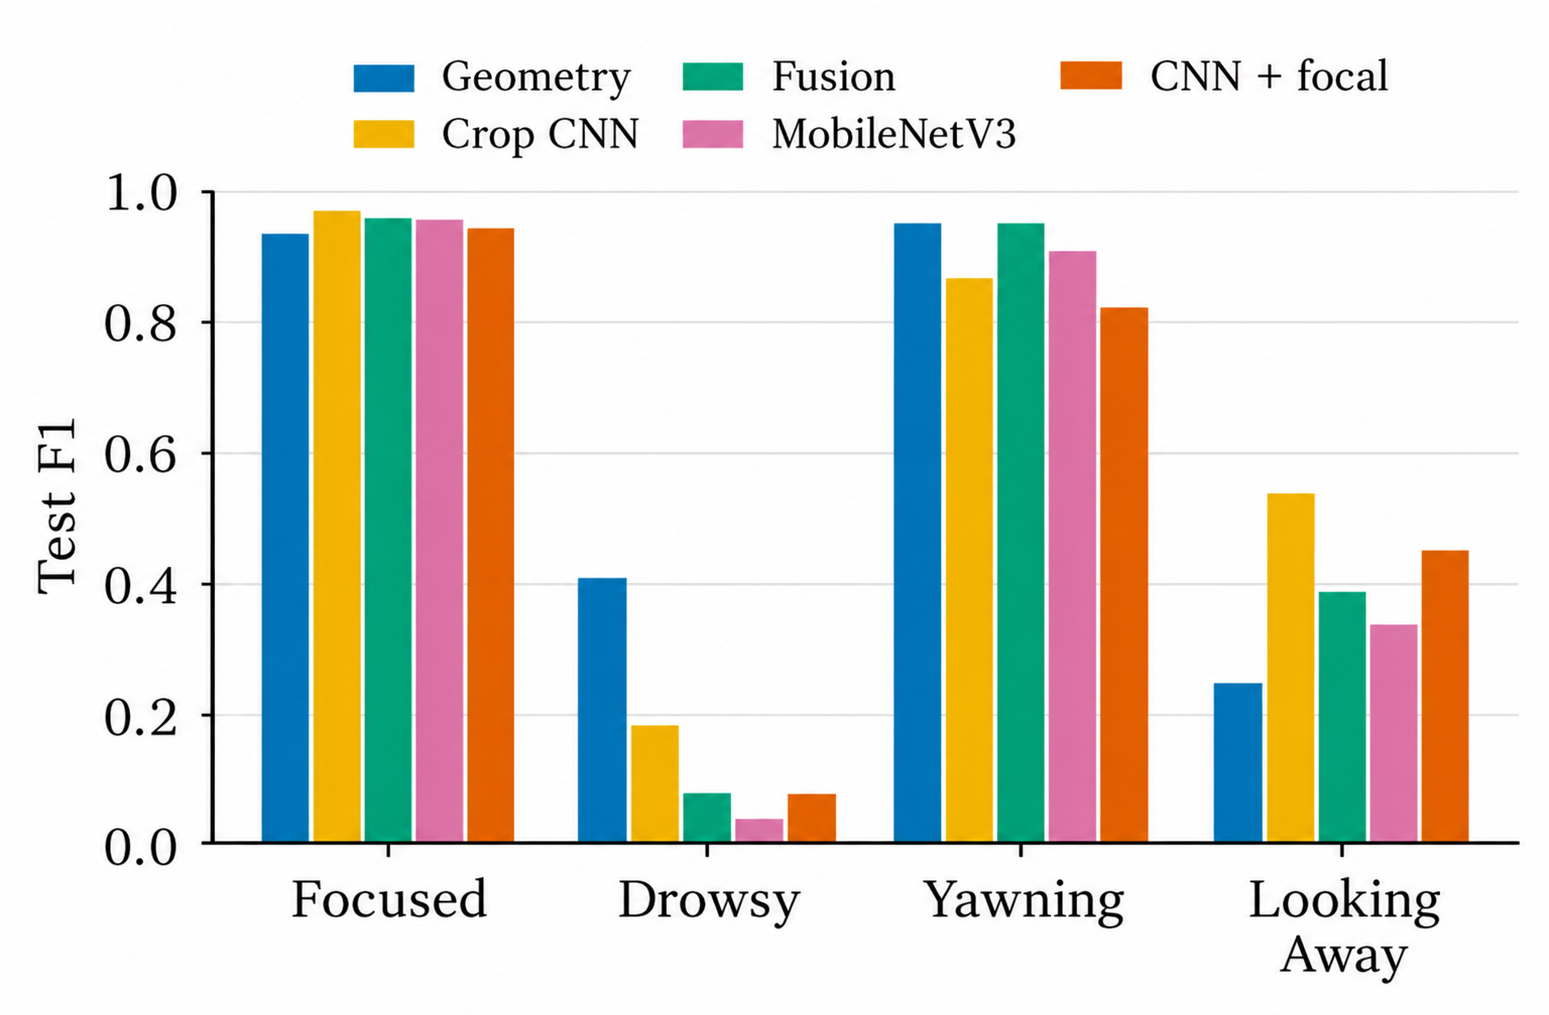
\includegraphics[width=\columnwidth]{test_f1_graph.png}
    \caption{Per-class test F1-scores of the five models (values in Table~\ref{tab:test_results}).}
    \label{fig:test_f1_comparison}
\end{figure}

\subsection{Effect of Manual Label Refinement}\label{sec:manualeffect}
We trained a separate Crop CNN on the manually refined labels of Section~\ref{sec:manualref} and evaluated it on the test split, using the same settings, split and seed as the main model. It reached a test accuracy of 0.604 and a macro-F1 of 0.431 (Table~\ref{tab:test_results}); the per-class F1 scores were 0.724 for Focused, 0.122 for Drowsy, 0.452 for Yawning and 0.427 for Looking Away and the best validation macro-F1 was 0.614 at epoch 8. For this run MAR-based relabeling of yawning clips was disabled, to isolate the effect of manual label refinement and avoid mixing two different label-correction methods. The correct reference is therefore the model trained without MAR relabeling (macro-F1 0.449), not the main Crop CNN (0.637). Relative to that model, macro-F1 changed by $-0.018$: Drowsy F1 rose from 0.088 to 0.122, while Yawning (0.472 to 0.452) and Looking Away (0.524 to 0.427) fell. With a single seed this difference is within the run-to-run variation we expect, so correcting 620 labels gave no measurable gain. Note that the manual correction also changed test labels, so the two test sets differ slightly.

\subsection{Low-Light Robustness}\label{sec:lowlightres}
Under darkening, we expect Face Mesh to fail before the classifier does. Face Mesh finds a face in 21,872 of the 22,064 L1 frames (99.1\%), 20,556 at L2 (93.2\%) and only 1,159 at L3 (5.3\%), against 21,874 on the clean test split (99.1\%). On the frames in which a face is still found, the selected Crop CNN reaches macro-F1 0.633, 0.568 and 0.466 on L1, L2 and L3 (accuracy 0.923, 0.897 and 0.750), against 0.637 on the clean test split; the INT8 model gives 0.631, 0.570 and 0.464. Frames without a face cannot be classified by any of our models, so accuracy on the remaining frames flatters the system and macro-F1 is the more honest measure. Because only 1,159 frames remain at L3, those scores are noisy; for example, FP32 MobileNetV3 scores higher on L3 (0.625) than on clean data (0.561). At L3 the application would lose the face in about 95\% of the frames and report Looking Away for them. In the application, a lost face is handled by the temporal layer, which reports Looking Away after 15 missing frames; this keeps the driver from being silently ignored, but it cannot distinguish a dark cabin from a driver who has turned away.

\subsection{Quantization and Benchmarks}\label{sec:quant}
Table~\ref{tab:fp32_int8_benchmark} compares FP32 and INT8 models under the protocol of Section~\ref{sec:quantprotocol}. Quantizing the Crop CNN reduces the checkpoint from 0.572 to 0.195 MB ($2.9\times$) and leaves accuracy unchanged: macro-F1 is 0.638 against 0.637 on the clean test split and 0.464 against 0.466 on L3. It does not make the model faster on this CPU: the model-only latency is 2.10 ms for INT8 against 1.33 ms for FP32. This is consistent with reports that the speed-up of INT8 inference depends on the integer instructions of the CPU \cite{shin2026}. The collapse of MobileNetV3 under INT8 is also in line with the finding that layers differ strongly in their sensitivity to quantization, which is why mixed-precision schemes keep sensitive layers in higher precision \cite{ramp2026}. The encoders are very small ($64\times64$ inputs, batch size one, one thread), so the quantize and dequantize steps cost about as much as the integer arithmetic saves. Run-to-run variation is large (in repeated runs, FP32 latency ranged from 1.18 to 2.36 ms), and process memory (RSS) varied by more between repeated runs than between precisions, so we draw no conclusion from the latency and memory differences. End-to-end, the pipeline runs at 95.0 FPS (10.5\,ms per frame) in FP32 and 87.9 FPS (11.4\,ms) in INT8 on one test clip; Face Mesh accounts for about 9\,ms of this. A speed-up from INT8 therefore remains to be tested on an ARM device with the qnnpack backend. The same procedure applied to MobileNetV3 (FX graph mode) shrinks it from 7.99 to 2.54\,MB ($3.1\times$) but damages it: macro-F1 falls from 0.561 to 0.480 on the clean test split and from 0.625 to 0.061 on L3, and latency rises from 5.0 to 9.1\,ms (medians of three runs). Hard-swish and squeeze-and-excitation layers are known to quantize poorly with simple post-training calibration; quantization-aware training or keeping those layers in FP32 would be needed. Even in FP32, MobileNetV3 is $14\times$ larger and $3.8\times$ slower than the Crop CNN, which supports the choice of the Crop CNN for deployment.

\subsection{Real-Time Application}\label{sec:realtime}
The demo runs the INT8 crop CNN on the Face Mesh crops, overlays landmarks, EAR, MAR and yaw, the smoothed state, PERCLOS and the frame rate on the webcam image, and plays an alarm when the temporal layer fires. The geometric values are displayed but not used for classification. End-to-end throughput is given in Section~\ref{sec:quant} (87.9 FPS with the INT8 model); this is processing speed, since the webcam delivers 30 fps.
The same temporal layer is also available in a browser version. The page opens the webcam, sends JPEG frames to a Flask server running on the same machine, which applies the identical Face Mesh, crop CNN and temporal layer and returns the state, EAR, MAR, yaw, pitch, PERCLOS and the count of blinks and yawns to be displayed. A blink is counted when EAR stays below the rule-based threshold (0.26) for between 0.05 and 1.0 s and a yawn when the smoothed state changes to Yawning. The page turns red and beeps while the state is Drowsy and also for Yawning and Looking Away. The browser version transmits fewer frames per second than the desktop one, so the frame-count rules take longer in seconds; we did not benchmark its throughput or latency and the numbers in this paper refer to the desktop pipeline. Neither version 


\vspace{0.2cm}
\section{Discussion and Limitations}

\textbf{Label quality limits every class.} Clip-level labeling introduces dataset noise, in line with the general finding that noisy labels harm generalization \cite{song2023} and with the frame-level re-annotation of YawDD \cite{mujtaba2025}. We therefore manually corrected 620 Drowsy and Looking Away labels in our recordings (Section~\ref{sec:manualref}). Under the same setting without MAR relabeling, the refined-label CNN reached macro-F1 0.431 against 0.449 for the original labels, so the correction gave no measurable gain (Drowsy F1 rose from 0.088 to 0.122, Looking Away fell from 0.524 to 0.427). Only a subset of frames from a few subjects was corrected, so remaining noise and the overlap between the Drowsy and Looking Away definitions probably dominate. Consistent annotation of all four classes with clear behavioral definitions is needed, but automatic correction from EAR or head-pose thresholds should be avoided, because the baseline uses the same features and the evaluation would become circular.
\newline
\textbf{Drowsy remains weak and the alarm depends on it.} The original selected model recognizes only 13\% of the Drowsy frames and the manual-refinement experiment does not resolve this problem. The refined-label CNN achieves a Drowsy F1 score of 0.122, so label corrections of this size alone do not guarantee improved Drowsy recognition. Because the alarm of the temporal layer counts Drowsy predictions, its sensitivity is limited by this recall. A PERCLOS signal computed directly from EAR, which the geometry network exploits (41\% recall) or a separate eye-closure classifier, is a natural alternative. Class definitions that separate a drooping head from looking down and more recordings of Drowsy with the head upright would also help.
\newline
\textbf{Why fusion did not help.} We can only offer hypotheses. The geometry features are partly redundant with the crops and the geometry branch makes the model rely on MAR and head pose, which cause the over-prediction of Looking Away. Large changes in per-class behavior between otherwise similar models (e.g. fusion and the Crop CNN) also suggest that results depend strongly on a small number of own subjects. With a single seed and a single split we cannot separate these effects; leave-one-subject-out cross-validation and several seeds would give more reliable estimates.
\newline
\textbf{Imbalance and capacity.} Focal loss and a larger encoder did not help on top of class-weighted cross-entropy, although both are widely recommended for imbalanced data \cite{lin2017,ghosh2024}. This suggests that the bottleneck is the amount and quality of the Drowsy and Looking Away data rather than the loss or the model size.
\newline
\textbf{Excluded frames and evaluation.} Frames without a detected face are excluded from training and evaluation. They include some of the clearest Looking Away examples (head turned far away), so the reported Looking Away F1 understates what the full system, with its no-face rule, can recognize. Drowsiness is also a temporal phenomenon: frame-level F1 is a harsh metric for a system whose alarm needs 1.5 s of consecutive evidence or a high PERCLOS and evaluating alarms on whole clips (detection delay and false alarms per minute) would match the intended use better.
\newline
\textbf{Subjects and sources.} Drowsy and Looking Away come from only 10 own subjects and 8 YouTube subjects, the test Looking Away frames from 2 own test subjects and the source mix differs between validation and test (Section~\ref{sec:split}). A model could also learn source-specific appearance (for example, YouTube frames occur only with Drowsy or only with Looking Away in a given split). Results for these two classes should therefore be read as indicative.
\newline
\textbf{Domain gap.} MRL Eye is infrared, YawDD is recorded inside vehicles and the demo uses a laptop webcam. Only the own recordings match the deployment domain and the eye-encoder initialization from MRL is a weak prior at best. This limitation is common: most driver-monitoring studies are run in simulators or laboratories \cite{john2024} and vision-only models generalize poorly to real driving conditions \cite{dontoh2025}.



\vspace{0.2cm}
\section{Conclusion}

We presented a lightweight four-state driver monitor built on MediaPipe Face Mesh, with a subject-disjoint data protocol and a quantization-oriented evaluation. A small crop CNN of about 138k parameters performed best (macro-F1 0.637, accuracy 91.2\%), narrowly ahead of a 3.7k-parameter geometry network; fusing both, a MobileNetV3 encoder and focal loss did not improve it. Most frames in yawning clips show a closed mouth: a CNN trained and evaluated on the unrefined labels reaches only 0.449 macro-F1 on that noisier label set. Manual refinement of 620 Drowsy and Looking Away labels brought no measurable gain under the same setting (0.431), pointing to remaining annotation noise and class ambiguity. Drowsy remained the hardest class and is mostly confused with Looking Away. INT8 quantization makes the Crop CNN $2.9\times$ smaller without loss of accuracy, but gives no speed-up on an x86 CPU, where Face Mesh dominates the run time; it degrades MobileNetV3, which supports the simpler encoder. Future work includes more participants and cleaner labels for Drowsy and Looking Away, cross-subject validation over several seeds, a PERCLOS signal based on eye geometry, clip-level alarm evaluation, infrared or multimodal sensing \cite{kim2023,knapik2024,dontoh2025}, a separate evaluation on real low-light recordings and deployment on an embedded ARM board or microcontroller, where INT8 inference can be expected to matter more \cite{alajlan2023,ramp2026}.



\vspace{0.2cm}
\section*{Acknowledgment}

The authors would like to thank the volunteers who helped in recording the webcam clips used in this project. They also acknowledge the creators of the MRL Eye and YawDD datasets.



\vspace{0.2cm}
\begin{thebibliography}{00}
\bibitem{fonseca2025} T. Fonseca and S. Ferreira, ``Drowsiness detection in drivers: A systematic review of deep learning-based models,'' \emph{Appl. Sci.}, vol. 15, no. 16, Art. no. 9018, 2025, doi: 10.3390/app15169018. 
\bibitem{fu2024} B. Fu, F. Boutros, C.-T. Lin, and N. Damer, ``A survey on drowsiness detection -- Modern applications and methods,'' arXiv:2408.12990, 2024 (accepted for publication in \emph{IEEE Trans. Intell. Veh.}).
\bibitem{fu2024app} S. Fu, Z. Yang, Y. Ma, Z. Li, L. Xu, and H. Zhou, ``Advancements in the intelligent detection of driver fatigue and distraction: A comprehensive review,'' \emph{Appl. Sci.}, vol. 14, no. 7, Art. no. 3016, 2024, doi: 10.3390/app14073016.
\bibitem{wang2023} J. Wang, W. Li, F. Li, J. Zhang, Z. Wu, Z. Zhong, and N. Sebe, ``100-Driver: A large-scale, diverse dataset for distracted driver classification,'' \emph{IEEE Trans. Intell. Transp. Syst.}, vol. 24, no. 7, pp. 7061--7072, 2023, doi: 10.1109/TITS.2023.3255923.
\bibitem{dontoh2025} A. Dontoh, S. Ivey, L. Sirbaugh, A. Danyo, and A. Aboah, ``Visual dominance and emerging multimodal approaches in distracted driving detection: A review of machine learning techniques,'' arXiv:2505.01973, 2025. 
\bibitem{mrl} Media Research Lab, VSB -- Technical University of Ostrava, ``MRL Eye Dataset.'' [Online]. Available: https://mrl.cs.vsb.cz/eyedataset.html. Accessed: Nov. 20, 2026.
\bibitem{fusek2018} R. Fusek, ``Pupil localization using geodesic distance,'' in \emph{Advances in Visual Computing (ISVC)}. Springer, 2018, doi: 10.1007/978-3-030-03801-4\_38. 
\bibitem{yawdd} S. Abtahi, M. Omidyeganeh, S. Shirmohammadi, and B. Hariri, ``YawDD: A yawning detection dataset,'' in \emph{Proc. 5th ACM Multimedia Systems Conf. (MMSys)}, Singapore, 2014, pp. 24--28, doi: 10.1145/2557642.2563678.
\bibitem{mujtaba2025} A. Mujtaba, M. Masana, G. Radchenko, and R. Prodan, ``YawDD+: Frame-level annotations for accurate yawn prediction,'' arXiv:2512.11446, 2025.
\bibitem{kapoor2023} S. Kapoor and A. Narayanan, ``Leakage and the reproducibility crisis in machine-learning-based science,'' \emph{Patterns}, vol. 4, no. 9, Art. no. 100804, 2023, doi: 10.1016/j.patter.2023.100804. 
\bibitem{alajlan2023} N. N. Alajlan and D. M. Ibrahim, ``DDD TinyML: A TinyML-based driver drowsiness detection model using deep learning,'' \emph{Sensors}, vol. 23, no. 12, Art. no. 5696, 2023, doi: 10.3390/s23125696. 
\bibitem{perclos} D. F. Dinges and R. Grace, ``PERCLOS: A valid psychophysiological measure of alertness as assessed by psychomotor vigilance,'' Federal Highway Administration, Office of Motor Carriers, Tech. Rep. FHWA-MCRT-98-006, 1998. 
\bibitem{soukupova2016} T. Soukupov\'a and J. \v{C}ech, ``Real-time eye blink detection using facial landmarks,'' in \emph{Proc. 21st Computer Vision Winter Workshop (CVWW)}, Rimske Toplice, Slovenia, 2016.
\bibitem{albadawi2022} Y. Albadawi, M. Takruri, and M. Awad, ``A review of recent developments in driver drowsiness detection systems,'' \emph{Sensors}, vol. 22, no. 5, Art. no. 2069, 2022, doi: 10.3390/s22052069.
\bibitem{rao2024} S. Janardhana Rao, V. S. K. Rupani, V. V. S. Thushar, and K. Tejith, ``Real-time drowsiness detection using eye aspect ratio and facial landmark detection,'' arXiv:2408.05836, 2024.
\bibitem{khan2026} F. Khan, S. Sharma, and M. R. Arulalan, ``Development of low-cost real-time driver drowsiness detection system using eye center tracking and dynamic thresholding,'' arXiv:2609.13756, 2026. 
\bibitem{kim2023} D. Kim \emph{et al.}, ``Real-time driver monitoring system with facial landmark-based eye closure detection and head pose recognition,'' \emph{Sci. Rep.}, vol. 13, Art. no. 18264, 2023, doi: 10.1038/s41598-023-44955-1. 
\bibitem{knapik2024} M. Knapik, B. Cyganek, and T. Balon, ``Multimodal driver condition monitoring system operating in the far-infrared spectrum,'' \emph{Electronics}, vol. 13, no. 17, Art. no. 3502, 2024, doi: 10.3390/electronics13173502. 
\bibitem{akhmedov2025} F. Akhmedov, H. Khujamatov, H.-S. Jeon \emph{et al.}, ``Joint driver state classification approach: Face classification model development and facial feature analysis improvement,'' \emph{Sensors}, vol. 25, no. 5, Art. no. 1472, 2025, doi: 10.3390/s25051472. 
\bibitem{john2024} Joel John M., Dinakaran K., Kavin F., Anitha P., Gurupandi D., and Pradeepa K., ``Enhanced generalization performance in deep learning for monitoring driver distraction: A systematic review,'' \emph{J. Adv. Res. Appl. Sci. Eng. Technol.}, vol. 48, no. 1, pp. 137--151, 2024, doi: 10.37934/araset.48.1.137151. 
\bibitem{weng2016} C.-H. Weng, Y.-H. Lai, and S.-H. Lai, ``Driver drowsiness detection via a hierarchical temporal deep belief network,'' in \emph{Computer Vision -- ACCV 2016 Workshops}, ser. Lecture Notes in Computer Science, vol. 10118. Cham, Switzerland: Springer, 2017, doi: 10.1007/978-3-319-54526-4\_9.
\bibitem{lugaresi2019} C. Lugaresi \emph{et al.}, ``MediaPipe: A framework for building perception pipelines,'' arXiv:1906.08172, 2019.
\bibitem{kartynnik2019} Y. Kartynnik, A. Ablavatski, I. Grishchenko, and M. Grundmann, ``Real-time facial surface geometry from monocular video on mobile GPUs,'' arXiv:1907.06724, 2019.
\bibitem{howard2019} A. Howard \emph{et al.}, ``Searching for MobileNetV3,'' in \emph{Proc. IEEE/CVF Int. Conf. Computer Vision (ICCV)}, 2019, pp. 1314--1324. 
\bibitem{qin2024} D. Qin \emph{et al.}, ``MobileNetV4: Universal models for the mobile ecosystem,'' in \emph{Computer Vision -- ECCV 2024}, 2024, doi: 10.1007/978-3-031-73661-2\_5. 
\bibitem{lin2017} T.-Y. Lin, P. Goyal, R. Girshick, K. He, and P. Doll\'ar, ``Focal loss for dense object detection,'' in \emph{Proc. IEEE Int. Conf. Computer Vision (ICCV)}, 2017, pp. 2980--2988. 
\bibitem{ghosh2024} K. Ghosh, C. Bellinger, R. Corizzo, P. Branco, B. Krawczyk, and N. Japkowicz, ``The class imbalance problem in deep learning,'' \emph{Mach. Learn.}, vol. 113, pp. 4845--4901, 2024, doi: 10.1007/s10994-022-06268-8. 
\bibitem{jacob2018} B. Jacob \emph{et al.}, ``Quantization and training of neural networks for efficient integer-arithmetic-only inference,'' in \emph{Proc. IEEE/CVF Conf. Computer Vision and Pattern Recognition (CVPR)}, 2018, pp. 2704--2713. 
\bibitem{krishnamoorthi2018} R. Krishnamoorthi, ``Quantizing deep convolutional networks for efficient inference: A whitepaper,'' arXiv:1806.08342, 2018. 
\bibitem{rokh2023} B. Rokh, A. Azarpeyvand, and A. Khanteymoori, ``A comprehensive survey on model quantization for deep neural networks in image classification,'' \emph{ACM Trans. Intell. Syst. Technol.}, vol. 14, no. 6, pp. 1--50, 2023, doi: 10.1145/3623402.
\bibitem{shin2026} Y. Shin, ``Is INT8 portable? A cross-platform measurement study of quantized inference on embedded and automotive accelerators,'' arXiv:2609.16085, 2026. 
\bibitem{ramp2026} D. Poblaci\'on-Criado, D. Garcia-Gasulla, and E. Quinones, ``RAMP: Robust adaptive mixed-precision quantization for edge CPU vision models,'' arXiv:2609.28262, 2026 (to appear in \emph{Proc. British Machine Vision Conf.}, 2026). 
\bibitem{song2023} H. Song, M. Kim, D. Park, Y. Shin, and J.-G. Lee, ``Learning from noisy labels with deep neural networks: A survey,'' \emph{IEEE Trans. Neural Netw. Learn. Syst.}, vol. 34, no. 11, pp. 8135--8153, Nov. 2023, doi: 10.1109/TNNLS.2022.3152527.
\bibitem{opencv} G. Bradski, ``The OpenCV library,'' \emph{Dr. Dobb's Journal of Software Tools}, 2000.
\bibitem{kingma2015} D. P. Kingma and J. Ba, ``Adam: A method for stochastic optimization,'' in \emph{Proc. Int. Conf. Learning Representations (ICLR)}, 2015. 
\bibitem{loshchilov2017} I. Loshchilov and F. Hutter, ``SGDR: Stochastic gradient descent with warm restarts,'' in \emph{Proc. Int. Conf. Learning Representations (ICLR)}, 2017. 
\bibitem{paszke2019} A. Paszke \emph{et al.}, ``PyTorch: An imperative style, high-performance deep learning library,'' in \emph{Advances in Neural Information Processing Systems (NeurIPS)}, vol. 32, 2019.
\bibitem{opitz2024} J. Opitz, ``A closer look at classification evaluation metrics and a critical reflection of common evaluation practice,'' \emph{Trans. Assoc. Comput. Linguist.}, vol. 12, pp. 820--836, 2024, doi: 10.1162/tacl\_a\_00675. 
\end{thebibliography}

\end{document}
